% 第1章第2节：范数、内积与完备性（函数范数与误差；范数收敛与Banach空间；内积与Hilbert空间）。

\section{范数、内积与完备性}
\label{sec:fs-norms-completeness}

有限维向量的范数与内积在卷一中已经建立，本节把它们用到函数上。定义本身几乎不变，变化在于用途：在无限维空间里，一列彼此越来越接近的元素是否真有极限、极限是否还在原来的集合中，需要逐一检查，而不再像有限维那样自动成立。

\subsection{函数范数与误差}
\label{sec:fs-norms}

\paragraph{两种误差要求}
比较$[0,1]$上的$f(x)=x$与$g(x)=x^2$，至少有两种自然的做法。若关心最坏的位置，可以取最大偏差$\sup_{x}|x-x^2|$；$x-x^2$在$x=\tfrac12$处取最大值，结果为$\tfrac14$。若关心整体的累计偏差，可以取$\int_0^1|x-x^2|\,dx=\tfrac12-\tfrac13=\tfrac16$。两个数都合理，回答的是不同的问题。为了让不同的误差规则共享同一套推理，我们只要求它们满足几条共同的性质。

\begin{definition}[范数]
\label{def:fs-norm}
设$V$是实（或复）线性空间。映射$\|\cdot\|:V\to[0,\infty)$称为$V$上的\term{范数}（norm），若对所有$f,g\in V$与标量$c$，
\begin{enumerate}
 \item 正定性：$\|f\|=0$当且仅当$f=0$；
 \item 齐次性：$\|cf\|=|c|\,\|f\|$；
 \item 三角不等式：$\|f+g\|\leq\|f\|+\|g\|$。
\end{enumerate}
配备了范数的线性空间称为赋范空间。
\end{definition}

三条公理各有用处。正定性保证误差为零当且仅当两个元素相同；齐次性保证把函数整体放大$c$倍时误差也放大$|c|$倍；三角不等式保证两段误差串联起来不超过各自之和，这是后面所有误差估计的基本工具。令$d(f,g)=\|f-g\|$，由三条公理可以直接验证度量公理（定义~\ref{def:metric-space}）：例如$d(f,h)=\|(f-g)+(g-h)\|\leq d(f,g)+d(g,h)$。所以每个赋范空间都是度量空间，第~\ref{chap:metric-spaces}章关于收敛、Cauchy列、闭集和完备性的结论都可以直接使用。

\paragraph{半范数与零方向}
有时一个误差公式满足齐次性和三角不等式，却让某些非零元素的“长度”为零，这样的公式称为\term{半范数}（seminorm）。在$[0,1]$上的全体有界可积函数中，$p(f)=\int_0^1|f|\,dx$就是半范数：上一节的$g=\mathbf 1_{\{1/2\}}$不为零，却有$p(g)=0$。又如在连续可微函数上，$p(f)=\sup_x|f'(x)|$对所有常数函数都取零。

处理零方向有两种办法。一是缩小对象：把$\int_0^1|f|\,dx$限制在$C([0,1])$上，若连续函数$f$在某点$x_0$处$|f(x_0)|>0$，则在$x_0$的一个邻域内$|f|>|f(x_0)|/2$，积分为正，所以在连续函数上它是范数。二是把零长度的元素识别为零，即对半范数为零的方向取商；在积分误差下，这正是第~\ref{sec:fs-ae-classes}小节的几乎处处等价类。第~\ref{sec:metric-pseudometric}节在度量空间中讨论过同样的商构造。无论哪种办法，都不能直接把只满足半范数条件的公式称为原对象上的范数。

\paragraph{系数误差与Gram矩阵}
回到章首的问题：当函数由有限个基函数表示时，函数之间的误差和系数之间的误差是什么关系？取平方积分误差$\|h\|_2^2=\int h^2\,d\mu$。对$f=\sum_jc_j\varphi_j$与$g=\sum_jc'_j\varphi_j$，记$\bm\delta=\bm c-\bm c'$，展开平方并利用积分的线性，
\[
 \|f-g\|_2^2=\int\Bigl(\sum_{i}\delta_i\varphi_i\Bigr)\Bigl(\sum_j\delta_j\varphi_j\Bigr)d\mu
 =\sum_{i,j}\delta_i\delta_j\int\varphi_i\varphi_j\,d\mu
 =\bm\delta^{\top}\bm G\bm\delta,
\]
其中$\bm G_{i,j}=\int\varphi_i\varphi_j\,d\mu$组成\term{Gram矩阵}（Gram matrix）。系数的欧氏距离平方是$\bm\delta^{\top}\bm\delta$，两者相等当且仅当$\bm G=\bm I$，即基函数两两正交且各自的平方积分为$1$。

在$[-1,1]$上取Lebesgue测度与基$\{1,x\}$，$\int1\,dx=2$，$\int x\,dx=0$，$\int x^2\,dx=\tfrac23$，所以$\bm G=\operatorname{diag}(2,\tfrac23)$，函数误差为$2\delta_1^2+\tfrac23\delta_2^2$。系数差$(1,0)$与$(0,1)$的欧氏长度都是$1$，对应的函数误差却分别是$\sqrt2$与$\sqrt{2/3}$。若改在$[0,1]$上使用同一组基，$\bm G=\begin{bmatrix}1&1/2\\1/2&1/3\end{bmatrix}$不再是对角阵，常数方向与线性方向的误差还会相互耦合。平方积分误差在连续函数上确实是范数：正定性的论证与上一段相同，三角不等式由Cauchy--Schwarz不等式得到，下面第~\ref{sec:fs-hilbert}小节在一般内积空间中给出证明。有限维的Gram矩阵、正交化与范数等价，可参考\BookChapterRef{chap:normed-inner-product-spaces}{卷一“赋范空间与内积空间”章}；本章不重建这些结论。

\subsection{范数收敛与Banach空间}
\label{sec:fs-banach}

有了范数，就可以讨论函数列的收敛。设$(f_n)$是赋范空间$V$中的序列，$f\in V$。若$\|f_n-f\|\to0$，称$f_n$\term{依范数收敛}（convergence in norm）到$f$。若对每个$\varepsilon>0$存在$N$，使$m,n\geq N$时$\|f_n-f_m\|<\varepsilon$，称$(f_n)$为范数意义下的\term{Cauchy列}（Cauchy sequence）。由三角不等式$\|f_n-f_m\|\leq\|f_n-f\|+\|f-f_m\|$，收敛列一定是Cauchy列。反过来是否成立，取决于空间。

\paragraph{斜坡逼近阶跃}
在$C([-1,1])$上使用平方积分范数$\|g\|_2=\bigl(\int_{-1}^1g^2\,dx\bigr)^{1/2}$，考察连续斜坡
\[
 g_n(x)=\begin{cases}-1,&x\leq-1/n,\\ nx,&|x|<1/n,\\ 1,&x\geq1/n,\end{cases}\qquad n\geq1 .
\]
图~\ref{fig:fs-ramp-step}画出了$g_2,g_4,g_{16}$：斜坡越来越陡，越来越像阶跃函数$\operatorname{sgn}$。我们先验证它们组成Cauchy列。设$m>n$。在$|x|\geq1/n$处$g_n=g_m$；在$|x|<1/n$处二者同号且绝对值不超过$1$，所以$|g_n-g_m|\leq1$。于是
\[
 \|g_n-g_m\|_2^2\leq\int_{-1/n}^{1/n}1\,dx=\frac2n\to0 .
\]

\begin{figure}[!htb]
  \centering
  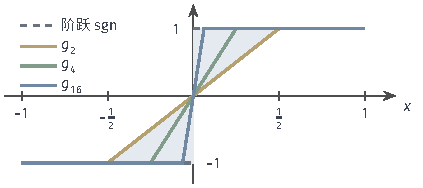
\includegraphics[width=71.6mm]{figures/02-abstract-mathematics/03-function-spaces/tikz/c1-ramp-step/figure.pdf}
  \caption{连续斜坡$g_n$逼近阶跃$\operatorname{sgn}$。$g_n$在$|x|\geq1/n$处与$\operatorname{sgn}$相同，只在宽为$2/n$的区间内线性过渡；阴影是$n=2$时二者的差所在的区域。直接积分得$\int_{-1}^1(g_n-\operatorname{sgn})^2\,dx=\tfrac{2}{3n}\to0$，但$\operatorname{sgn}$在$0$处跳跃，没有连续代表。}
  \label{fig:fs-ramp-step}
\end{figure}

接下来证明这列函数在$C([-1,1])$中没有$\|\cdot\|_2$极限。假设存在连续函数$g$使$\|g_n-g\|_2\to0$。任取$\delta\in(0,1)$，当$n>1/\delta$时$g_n$在$[\delta,1]$上恒为$1$，所以
\[
 \int_\delta^1(1-g)^2\,dx\leq\int_{-1}^1(g_n-g)^2\,dx\to0 .
\]
左边不依赖$n$，只能为零；$(1-g)^2$连续且非负，故$g=1$在$[\delta,1]$上处处成立。同理$g=-1$在$[-1,-\delta]$上成立。由于$\delta$任意，$g$在$(0,1]$上恒为$1$、在$[-1,0)$上恒为$-1$，在$0$处不可能连续，矛盾。

这个例子把两件事分开了：“各项互相接近”是序列自身的性质，“在给定的集合中存在极限”则同时取决于集合和范数。直观上，$g_n$的“极限”应该是阶跃函数，只是阶跃函数不在$C([-1,1])$中。

\begin{definition}[Banach空间]
\label{def:fs-banach}
若赋范空间$V$中的每个Cauchy列都依范数收敛到$V$中的某个元素，称$V$是\term{完备}（complete）的。完备的赋范空间称为\term{Banach空间}（Banach space）。
\end{definition}

按此定义，$(C([-1,1]),\|\cdot\|_2)$不是Banach空间。完备性同时依赖候选集合和范数：第~\ref{sec:fs-uniform-norm}小节将证明同一个$C([-1,1])$在最大偏差范数下完备，第~\ref{sec:fs-lp-completeness}小节则把集合扩大为可测函数的等价类，使平方积分范数下的极限有处可去。

\paragraph{闭子空间与完备性}
在已经完备的空间里，子空间是否完备由它是否闭决定。第~\ref{sec:metric-convergence-completeness}节对度量空间证明了：完备空间的闭子集是完备的，完备子集一定是闭的（定理~\ref{thm:metric-complete-closed}）。用在Banach空间$X$的线性子空间$M$上，这两句话的分工很清楚：$X$的完备性保证$M$中的Cauchy列在$X$中有极限，$M$的闭性保证这个极限没有跑出$M$。

多项式给出一个不闭的子空间。在$[0,1]$上用最大偏差衡量误差，$e^x$的Taylor多项式$p_N(x)=\sum_{k=0}^Nx^k/k!$满足
\[
 \sup_{x\in[0,1]}|e^x-p_N(x)|\leq\frac{e}{(N+1)!}\to0,
\]
这是Lagrange余项的估计。所以$p_N$是多项式空间中的Cauchy列，在连续函数空间中的极限是$e^x$，而$e^x$不是多项式（它的各阶导数都不恒为零）。多项式空间因此不闭，也不完备。第~\ref{sec:apx-polynomial}小节将说明，多项式在这个范数下可以逼近任意连续函数，即它的闭包是整个$C([0,1])$。

\paragraph{完备化}
不完备的空间可以通过添加极限补全。第~\ref{sec:metric-completion}节给出了度量空间的完备化（定理~\ref{thm:metric-completion}）：把Cauchy列$(f_n)$与$(g_n)$在$\|f_n-g_n\|\to0$时视为等价，等价类全体在距离$\lim_n\|f_n-g_n\|$下完备，原空间作为常数列等距地嵌入其中且稠密。对赋范空间，线性运算可以沿Cauchy列延拓：$[(f_n)]+[(g_n)]=[(f_n+g_n)]$，$c[(f_n)]=[(cf_n)]$，范数取$\lim_n\|f_n\|$。这个极限存在，因为$\bigl|\|f_n\|-\|f_m\|\bigr|\leq\|f_n-f_m\|$说明$(\|f_n\|)$是实数Cauchy列；三角不等式和齐次性在极限中保留，所以完备化是Banach空间。

抽象完备化只保证“存在一个完备空间把原空间作为稠密子空间”，并不告诉我们新元素是不是函数、是哪一类函数。把斜坡例子中的“新元素”识别为阶跃函数的等价类，需要第~\ref{sec:fs-integral}节的$L^2$空间和第~\ref{sec:fs-density-separability}小节的稠密性结论。因此本节不预先声称任何给定的函数类已经完备；后面的积分空间、Sobolev空间和核空间都会分别说明完备性从何而来。

\subsection{内积与Hilbert空间}
\label{sec:fs-hilbert}

平方误差还带来一种范数一般没有的结构：可以谈论两个函数是否“垂直”，从而把误差分解成互不干扰的分量。这需要内积。

\begin{definition}[实内积与Hilbert空间]
\label{def:fs-inner-product}
设$V$是实线性空间。映射$\langle\cdot,\cdot\rangle:V\times V\to\mathbb R$称为\term{内积}（inner product），若对所有$f,g,h\in V$与实数$a,b$，
\begin{enumerate}
 \item 对称性：$\langle f,g\rangle=\langle g,f\rangle$；
 \item 线性：$\langle af+bg,h\rangle=a\langle f,h\rangle+b\langle g,h\rangle$；
 \item 正定性：$\langle f,f\rangle\geq0$，且等号当且仅当$f=0$。
\end{enumerate}
记$\|f\|=\sqrt{\langle f,f\rangle}$。在这个范数下完备的内积空间称为\term{Hilbert空间}（Hilbert space）。
\end{definition}

$\|f\|=\sqrt{\langle f,f\rangle}$确实是范数，关键在三角不等式。对任意实数$t$，
\[
 0\leq\|f-tg\|^2=\|f\|^2-2t\langle f,g\rangle+t^2\|g\|^2 .
\]
若$g\neq0$，右边是$t$的二次函数且恒非负，判别式不大于零，得到\term{Cauchy--Schwarz不等式}（Cauchy--Schwarz inequality）
\begin{equation}
 |\langle f,g\rangle|\leq\|f\|\,\|g\| ;
 \label{eq:fs-cauchy-schwarz}
\end{equation}
$g=0$时两边都为零。再由$\|f+g\|^2=\|f\|^2+2\langle f,g\rangle+\|g\|^2\leq(\|f\|+\|g\|)^2$得到三角不等式。正定性与齐次性直接来自内积公理。所以内积空间都是赋范空间，Hilbert空间都是Banach空间。

\paragraph{积分正交}
在$C([-1,1])$上，$\langle f,g\rangle=\int_{-1}^1f(x)g(x)\,dx$是内积：对称性与线性来自积分的性质，正定性的论证与第~\ref{sec:fs-norms}小节相同。它诱导的范数正是平方积分范数$\|\cdot\|_2$。由斜坡例子，这个内积空间不完备，因而不是Hilbert空间；它在第~\ref{sec:fs-integral}节中的扩充$L^2([-1,1])$才是。

若$\langle f,g\rangle=0$，称$f$与$g$\term{正交}（orthogonal）。函数的正交由乘积的整体积分决定，与两条曲线在平面上相交的角度无关。图~\ref{fig:fs-integral-orthogonality}(a)中，$1$与$x$的乘积在正负半区间上的面积各为$\pm\tfrac12$，相加为零，二者正交；(b)中$1$与$x^2$的乘积处处非负，积分为$\tfrac23$，二者不正交。用同样的对称性还可以看出，$[-1,1]$上任何偶函数与任何奇函数都正交，这一事实将在第~\ref{sec:fs-orthonormal-bases}小节用到。

\begin{figure}[!htb]
  \centering
  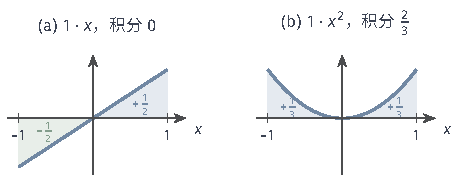
\includegraphics[width=78.2mm]{figures/02-abstract-mathematics/03-function-spaces/tikz/c1-integral-orthogonality/figure.pdf}
  \caption{积分内积下的正交。$[-1,1]$上取Lebesgue测度，曲线是两个函数的乘积，阴影面积带符号累计后即为内积。(a)$1\cdot x$的正负面积各为$\tfrac12$，内积为$0$，$1$与$x$正交；(b)$1\cdot x^2$处处非负，内积为$\tfrac23$，$1$与$x^2$不正交。正交与否只看积分，与曲线的倾角无关。}
  \label{fig:fs-integral-orthogonality}
\end{figure}

\paragraph{复内积的约定}
信号和频域表示需要复值函数。复线性空间上的内积改为共轭对称：$\langle g,f\rangle=\overline{\langle f,g\rangle}$，并且全书统一约定内积对第一个变量共轭线性、对第二个变量线性，即
\[
 \langle af,g\rangle=\bar a\langle f,g\rangle,\qquad \langle f,ag\rangle=a\langle f,g\rangle .
\]
积分内积相应写作$\langle f,g\rangle=\int\overline{f}\,g\,d\mu$。共轭不可省略：在$[-\pi,\pi]$上取$f(x)=e^{ix}$，若不取共轭，$\int f\cdot f\,dx=\int e^{2ix}\,dx=0$，一个非零函数的“长度”会是零；取共轭后$\langle f,f\rangle=\int|e^{ix}|^2\,dx=2\pi$。Cauchy--Schwarz不等式在复情形仍成立（把上面的$t$换成适当的复数），本章主线只用实内积。

\paragraph{范数何时来自内积}
内积诱导的范数满足\term{平行四边形恒等式}（parallelogram identity）
\[
 \|f+g\|^2+\|f-g\|^2=2\|f\|^2+2\|g\|^2,
\]
只需把两边按内积展开，交叉项相互抵消。一般的范数未必满足它。在$C([0,1])$上取最大偏差$\|f\|_\infty=\sup_x|f(x)|$，令$f=1$、$g=x$：$\|f+g\|_\infty=2$，$\|f-g\|_\infty=1$，左边为$5$；$\|f\|_\infty=\|g\|_\infty=1$，右边为$4$。所以最大偏差范数不来自任何内积，$C([0,1])$在这个范数下即使完备，也不是Hilbert空间。“有没有内积”和“是否完备”是两个独立的判断。

\paragraph{有限维直觉的边界}
在有限维空间中，任意两个范数等价，即存在常数$c,C>0$使$c\|v\|_a\leq\|v\|_b\leq C\|v\|_a$，所以范数的选择不影响收敛与完备性。这一结论不能搬到无限维。在$C([0,1])$上，$\|f\|_2\leq\|f\|_\infty$总成立（被积函数不超过$\|f\|_\infty^2$），反方向却没有常数：取$f_n(x)=x^n$，
\[
 \|x^n\|_\infty=1,\qquad \|x^n\|_2=\Bigl(\int_0^1x^{2n}\,dx\Bigr)^{1/2}=\frac{1}{\sqrt{2n+1}}\to0,
\]
比值$\|x^n\|_\infty/\|x^n\|_2=\sqrt{2n+1}$无界。同一个函数集合上的两个范数可以给出完全不同的收敛判断，斜坡例子中的完备性差异也由此而来。
